% ============================================================
%  7.5. EVALUACIÓN Y RESULTADOS  -- parte del capítulo 7
%  ------------------------------------------------------------
%  Archivo separado para que cada fase de CRISP-DM se pueda
%  editar y compilar por separado. Solo contenido: el formato,
%  los rótulos y las referencias los resuelve el preámbulo.
%  Los \label originales se conservan sin cambios.
% ============================================================
\section{Evaluación y Resultados}
\label{sec:evaluacion-resultados}

Esta sección documenta la quinta fase de CRISP-DM, ejecutada mediante cinco scripts
(\var{21_hypothesis_tests.py} a \var{28_ranking_explainer.py}) sobre las
predicciones de los cuatro modelos de la sección~\ref{sec:modelado}.

\subsection{Métricas y resultados por modelo}
\label{sec:resultados-modelo}

Se reportan tres métricas, cada una con un rol distinto dado que el objetivo es fuertemente
asimétrico (sección~\ref{sec:seleccion-algoritmos}): el \textbf{MAE} (error absoluto medio),
interpretable directamente en consultas por semana; el \textbf{RMSE}, que penaliza más los
errores grandes y es por tanto sensible a la presencia de valores extremos; y el
\textbf{R\textsuperscript{2}}, la proporción de varianza explicada respecto de predecir
siempre la media.

\begin{table}[htbp]
  \centering
  \caption{Desempeño comparado en el conjunto de prueba (8 semanas nunca vistas)}
  \label{tab:resultados-modelos}
  \interlineadoSimple
  \begin{tabular}{lrrr}
    \toprule
    \textbf{Modelo} & \textbf{MAE} & \textbf{RMSE} & \textbf{R\textsuperscript{2}} \\
    \midrule
    \textbf{Random Forest (final)} & \textbf{10,19} & \textbf{80,70} & \textbf{0,656} \\
    Base estacional (media móvil 4 sem.) & 11,05 & 85,70 & 0,613 \\
    Base ingenua (persistencia, $t-1$) & 11,30 & 91,90 & 0,555 \\
    XGBoost & 13,85 & 102,82 & 0,442 \\
    Lasso & 44,03 & 520,76 & $-13,305$ \\
    Ridge & 48,97 & 559,13 & $-15,491$ \\
    \bottomrule
  \end{tabular}
  \fuente{Elaboración propia, a partir de \var{19_model_comparison.py} ---
  \var{reports/03_modeling/02_model_comparison.md}.}
\end{table}

\begin{figure}[htbp]
  \centering
  \caption{Predicho vs. observado, Random Forest, conjunto de prueba}
  \label{fig:pred-vs-obs}
  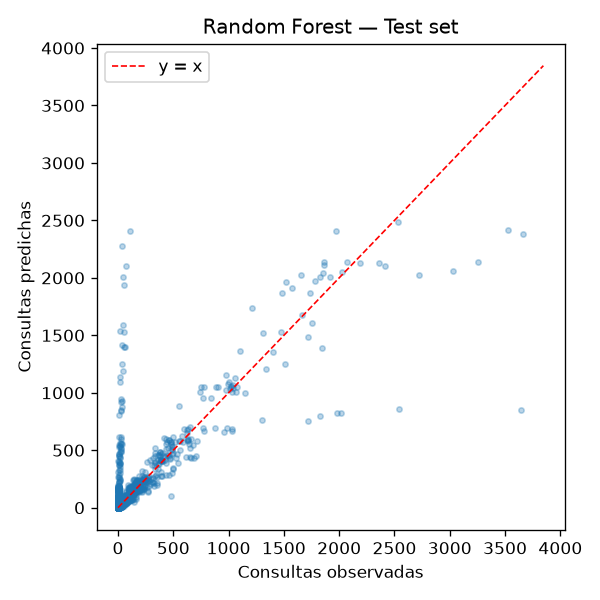
\includegraphics[width=0.7\textwidth]{imagenes/fig_pred_vs_obs_rf.png}
  \fuente{Elaboración propia, a partir de \var{19_model_comparison.py}.}
\end{figure}

\subsubsection{Hallazgo: inestabilidad de extrapolación de los modelos lineales}

Ridge y Lasso muestran R\textsuperscript{2} fuertemente negativo en prueba pese a un ajuste
razonable en entrenamiento (MAE de 30,06 y 25,57 respectivamente): 50 y 42 de las 12.416
predicciones de cada uno alcanzan el techo de seguridad de extrapolación impuesto sobre la
reversión \texttt{expm1} (sección~\ref{sec:tipo-problema}). La causa es la combinación de una
tendencia sostenida --\var{week_idx} toma en prueba valores nunca vistos en
entrenamiento-- con la asimetría extrema del objetivo (Gini~$=0{,}934$,
sección~\ref{sec:sensibilidad-h3}): un pequeño error en escala logarítmica se amplifica
exponencialmente al revertir la transformación. \textbf{No es un defecto de implementación:
es evidencia de que la relación entre demanda y condiciones territoriales no es lineal.} Los
modelos de árboles no sufren este problema porque sus predicciones están acotadas por los
valores observados en las hojas de entrenamiento.

\subsection{Sobreajuste y subajuste}
\label{sec:sobreajuste}

\begin{table}[htbp]
  \centering
  \caption{Brecha entre entrenamiento y prueba (MAE)}
  \label{tab:brecha-train-test}
  \interlineadoSimple
  \begin{tabular}{lrrr}
    \toprule
    \textbf{Modelo} & \textbf{MAE entrenamiento} & \textbf{MAE prueba} & \textbf{Brecha} \\
    \midrule
    Random Forest & 2,19 & 10,19 & $+8,00$ \\
    XGBoost & 2,09 & 13,85 & $+11,76$ \\
    Lasso & 25,57 & 44,03 & $+18,46$ \\
    Ridge & 30,06 & 48,97 & $+18,92$ \\
    \bottomrule
  \end{tabular}
  \fuente{Elaboración propia, a partir de \var{19_model_comparison.py}.}
\end{table}

La brecha de Random Forest ($+8{,}00$) es menor que la de XGBoost ($+11{,}76$) pese a
hiperparámetros de complejidad similar, señal de menor sobreajuste relativo. Las curvas de
aprendizaje --Random Forest reentrenado con tamaños de entrenamiento crecientes, evaluado
contra una ventana de validación de 13 semanas no vista-- refuerzan esta lectura.

\begin{figure}[htbp]
  \centering
  \caption{Curva de aprendizaje de Random Forest}
  \label{fig:curva-aprendizaje}
  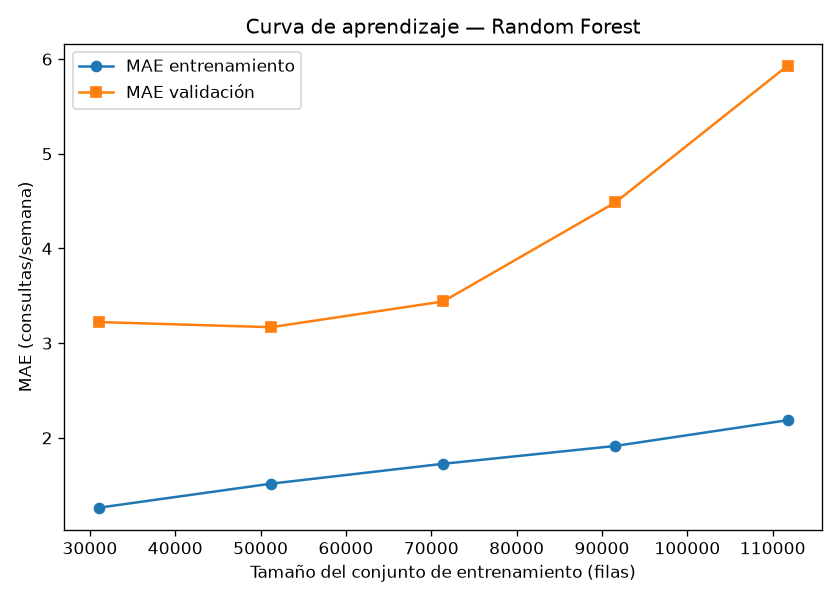
\includegraphics[width=0.7\textwidth]{imagenes/fig_learning_curve.png}
  \fuente{Elaboración propia, a partir de \var{23_error_analysis.py} ---
  \var{reports/04_evaluation/03_error_analysis.md}.}
\end{figure}

La brecha entrenamiento-validación crece de forma moderada a medida que aumenta el tamaño de
entrenamiento ($+1{,}96 \to +1{,}65 \to +1{,}71 \to +2{,}57 \to +3{,}74$), con un MAE de
entrenamiento que se mantiene bajo (1,26 a 2,19) mientras el de validación oscila en un rango
razonable (3,2 a 5,9): la firma esperada de un árbol de profundidad acotada
(\var{max_depth}$=10$) que ajusta ruido de forma limitada, sin señal de varianza
descontrolada. La curva tiene solo cinco puntos por costo computacional --cada uno reentrena
un modelo completo--, suficiente para descartar sobreajuste severo pero no para un
diagnóstico fino.

\subsection{Contraste de hipótesis}
\label{sec:contraste-hipotesis}

\subsubsection{H1 --- Brecha de cobertura centro-periferia}

Se contrasta si las celdas periféricas (mayor distancia al centro) tienen una tasa de
demanda no resuelta (\var{pct_uncovered_orig}) significativamente mayor que las
centrales. La unidad de análisis es la \textbf{celda}, no la celda-semana: se promedia
\var{pct_uncovered_orig} sobre todas las semanas de cada celda, porque tratar cada
semana como observación independiente constituiría pseudorreplicación --inflaría el tamaño
muestral de 1.552 a decenas de miles y produciría un valor p espuriamente pequeño. Los
grupos se definen por la mediana de \var{dist_center_km} (15,49~km): 776 celdas
centrales y 776 periféricas, un corte simple y documentado pero arbitrario, que no
corresponde a ningún límite administrativo real.

\begin{table}[htbp]
  \centering
  \caption{Contraste H1: tasa de demanda no resuelta por grupo territorial}
  \label{tab:h1-resultado}
  \interlineadoSimple
  \begin{tabular}{lrr}
    \toprule
    \textbf{Grupo} & \textbf{n celdas} & \textbf{Media \var{pct_uncovered_orig}} \\
    \midrule
    Central & 776 & 0,213 \\
    Periferia & 776 & 0,351 \\
    \bottomrule
  \end{tabular}
  \fuente{Elaboración propia, a partir de \var{21_hypothesis_tests.py} ---
  \var{reports/04_evaluation/01_hypothesis_tests.md}.}
\end{table}

La prueba de Shapiro-Wilk rechazó la normalidad en ambos grupos ($p=2{,}18\times10^{-41}$ en
el centro, $p=1{,}423\times10^{-38}$ en la periferia) --resultado esperable, dado que la
variable es una proporción con masa concentrada en 0 y 1--, lo que fundamenta el uso de la
prueba U de Mann-Whitney, no paramétrica. El resultado es concluyente: estadístico
$341{.}618{,}0$, $p=6{,}101\times10^{-9}$, significativo a $\alpha=0{,}05$, con una
correlación biserial por rangos de $-0{,}135$ (tamaño de efecto pequeño, dado el tamaño
muestral). \textbf{Se confirma H1}: las celdas periféricas tienen una tasa de demanda no
resuelta significativamente mayor que las centrales.

\subsubsection{H2 --- Random Forest frente a la línea base estacional}

Se contrasta si el error del modelo final es significativamente menor que el de la media
móvil de 4 semanas. El test de Diebold-Mariano, diseñado específicamente para comparar
exactitud predictiva entre dos modelos sobre una serie temporal, opera sobre la serie
semanal de 8 puntos de prueba: con esa potencia insuficiente por construcción, el resultado
no es significativo (estadístico $-0{,}705$, $p=0{,}503$). Un resultado no significativo no
implica equivalencia entre los modelos, solo que ocho semanas no alcanzan para distinguirlos
con confianza; la ventana de prueba se fijó en la sección~\ref{sec:particion-cronologica}
para preservar datos de entrenamiento, no para maximizar la potencia de este contraste.

Se complementa con una prueba de Wilcoxon de rangos con signo, pareada por celda (1.552
observaciones, potencia suficiente): estadístico $287.045{,}0$, $p=0{,}0326$, significativo.
A primera vista esto contradice que Random Forest solo supere a la base en el 31,0~\% de las
celdas; la explicación está en la magnitud, no en el conteo:

\begin{table}[htbp]
  \centering
  \caption{Dónde gana cada método (test de Wilcoxon pareado por celda)}
  \label{tab:h2-desglose}
  \interlineadoSimple
  \begin{tabularx}{\textwidth}{@{}Xrrr@{}}
    \toprule
    \textbf{Grupo} & \textbf{n celdas} & \textbf{Dif. media (RF $-$ base)} & \textbf{Demanda media} \\
    \midrule
    Gana Random Forest & 481 & $-3,72$ & 42,9 consultas/sem. \\
    Gana la base estacional & 632 & $+0,71$ & 13,8 consultas/sem. \\
    Empate exacto & 439 & --- & --- \\
    \bottomrule
  \end{tabularx}
  \fuente{Elaboración propia, a partir de \var{21_hypothesis_tests.py}.}
\end{table}

Random Forest gana por un margen grande en celdas de alta demanda y pierde por un margen
pequeño en celdas casi sin actividad. \textbf{Se confirma H2, con matices}: la ventaja de
Random Forest sobre la línea base es estadísticamente significativa y está concentrada
exactamente en las celdas de mayor demanda --el segmento operativamente más relevante--, no
distribuida de manera uniforme. Reportar solo el valor p o solo el porcentaje de celdas
ganadas habría sido engañoso en direcciones opuestas.

\subsection{Análisis de errores}
\label{sec:analisis-errores}

La media de residuos de Random Forest en prueba es $-4{,}758$. Esta cifra no debe calificarse
de sesgo despreciable: representa cerca de la mitad del MAE de prueba (10,19), lo que indica
una tendencia sistemática a la sobrepredicción, atribuible en buena parte a las semanas
parciales que se describen a continuación.

\begin{figure}[htbp]
  \centering
  \caption{Distribución de residuos por celda, conjunto de prueba}
  \label{fig:residuos}
  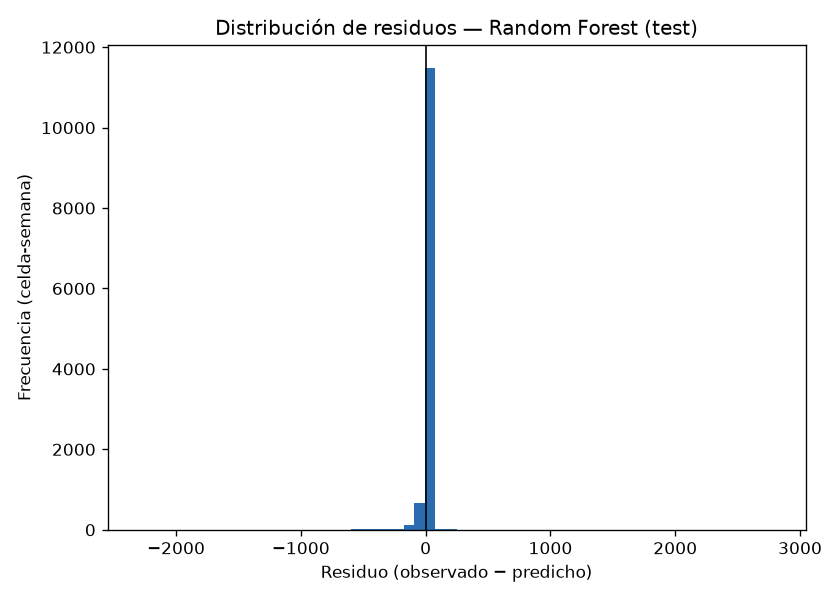
\includegraphics[width=0.65\textwidth]{imagenes/fig_residuals_by_cell.png}
  \fuente{Elaboración propia, a partir de \var{23_error_analysis.py}.}
\end{figure}

\subsubsection{Hallazgo: dos semanas de prueba son fragmentos de un día}
\label{sec:semanas-parciales}

Al construir la serie semanal agregada se detectó que la demanda observada total cae a
apenas 1--3~\% de una semana normal en dos de las ocho semanas de prueba: 2024-W18 (909
consultas, la semana de reanudación tras el vacío, con solo unas 5 horas de datos) y
2024-W23 (1.367 consultas, el corte final del dataset, con solo unas 11 horas de datos). No
se trata de semanas con demanda real más baja sino de fragmentos de un solo día --un
artefacto de cobertura de exportación no advertido al fijar la partición
(sección~\ref{sec:particion-cronologica}).

\begin{table}[htbp]
  \centering
  \caption{Impacto de las semanas parciales sobre las métricas del modelo final}
  \label{tab:semanas-parciales}
  \interlineadoSimple
  \begin{tabular}{lrrr}
    \toprule
    \textbf{Escenario} & \textbf{MAE} & \textbf{RMSE} & \textbf{R\textsuperscript{2}} \\
    \midrule
    Las 8 semanas de prueba (resultado principal) & 10,19 & 80,70 & 0,656 \\
    Las 6 semanas completas (sin las parciales) & 5,91 & 52,87 & 0,889 \\
    \bottomrule
  \end{tabular}
  \fuente{Elaboración propia, a partir de \var{23_error_analysis.py} ---
  \var{reports/04_evaluation/03_error_analysis.md}.}
\end{table}

Esta monografía reporta \textbf{ambas cifras juntas}, y no una sola. El MAE de 10,19 se
mantiene como resultado principal por ser la evaluación más conservadora y no requerir una
decisión de exclusión posterior a la observación de los datos; el MAE de 5,91 es la
estimación más representativa del desempeño en una semana calendario completa, y es
consistente con el historial de validación cruzada (2,8 a 6,2,
sección~\ref{sec:hiperparametros}), frente al cual 10,19 resulta atípico una vez comprendida
su causa. Presentar solo la segunda cifra sería selección posterior favorable; presentar solo
la primera ocultaría que el error está inflado por un artefacto identificado y rastreado
hasta el dato crudo.

\begin{figure}[htbp]
  \centering
  \caption{Estabilidad temporal del error semanal en el conjunto de prueba}
  \label{fig:estabilidad-error}
  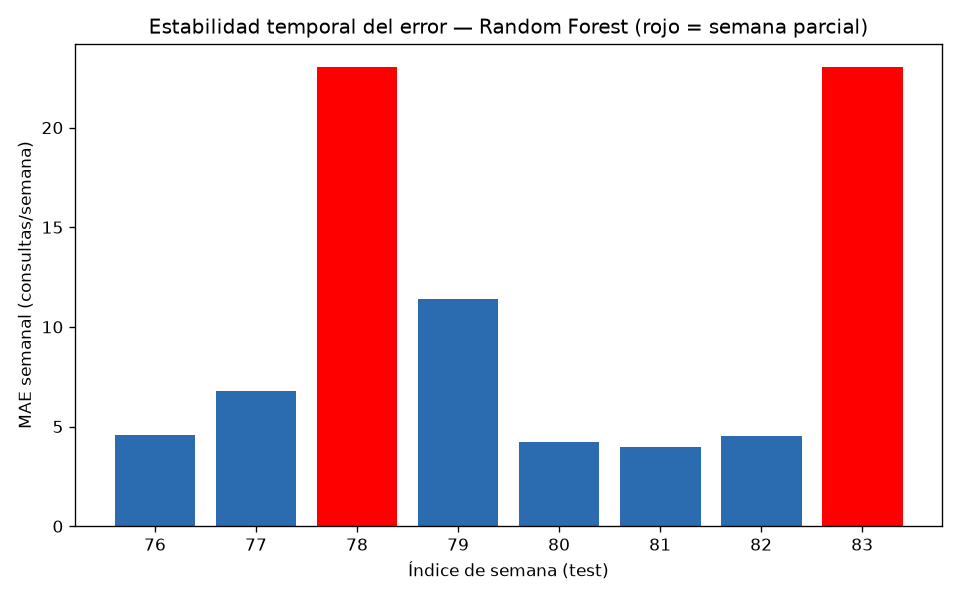
\includegraphics[width=0.7\textwidth]{imagenes/fig_weekly_error_stability.png}
  \fuente{Elaboración propia, a partir de \var{23_error_analysis.py}. Las semanas
  2024-W18 y 2024-W23 (parciales) se resaltan.}
\end{figure}

El artefacto no se limita a las dos semanas donde se originó: 2024-W19, la semana
inmediatamente posterior a 2024-W18, también registra un MAE elevado (11,38, más del doble de
la mediana de las semanas limpias) pese a no tener ningún problema de datos propio, porque
hereda de 2024-W18 un \var{lag1_n_queries_orig} artificialmente bajo (909 consultas en
vez de un nivel normal de más de 40.000). El horizonte de pronóstico evaluado no muestra
degradación progresiva por sí solo; la única inestabilidad detectada tiene una causa puntual
e identificada, no un problema estructural del modelo.

\subsection{Interpretación desde el problema original}
\label{sec:interpretacion-resultados}

La pregunta de investigación --cómo se distribuye la demanda de información de transporte no
resuelta y qué características del territorio se asocian con esa distribución-- se responde
con evidencia convergente de tres análisis. Primero, H1 confirma estadísticamente que la
brecha de cobertura es mayor en la periferia. Segundo, el gradiente espacial de demanda es
real: la correlación de Spearman entre \var{dist_center_km} y la demanda decae tanto
para la demanda observada ($\rho=-0{,}615$, $p=2{,}8\times10^{-162}$) como para la predicha
($\rho=-0{,}618$, $p=3{,}3\times10^{-164}$).

\begin{figure}[htbp]
  \centering
  \caption{Demanda semanal observada vs. distancia al centro}
  \label{fig:demanda-distancia}
  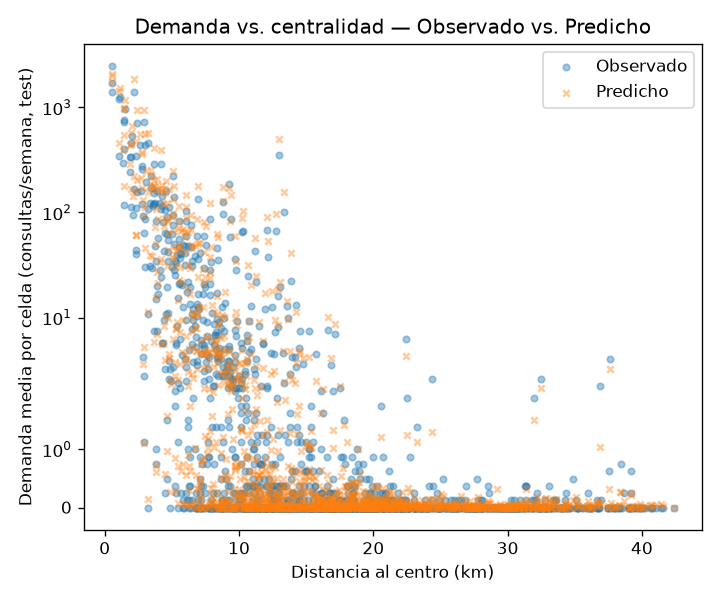
\includegraphics[width=0.7\textwidth]{imagenes/fig_demand_vs_distance.png}
  \fuente{Elaboración propia, a partir de \var{22_results_analysis.py} ---
  \var{reports/04_evaluation/02_results_analysis.md}.}
\end{figure}

Tercero, H2 muestra que el valor predictivo del modelo está concentrado exactamente donde
más importa operativamente: las celdas de mayor demanda. En conjunto, la periferia combina
\textbf{menor demanda absoluta} con \textbf{peor cobertura relativa} --un patrón consistente
con zonas de expansión urbana con transporte formal insuficiente, y no con una simple falta
de interés de los usuarios; debe recordarse, como se ha señalado en capítulos anteriores, que
``demanda'' significa aquí consultas de planificación --intención de viaje-- y no
desplazamientos confirmados.

\begin{figure}[htbp]
  \centering
  \caption{Demanda semanal agregada, observada vs. predicha (conjunto de prueba)}
  \label{fig:demanda-semanal}
  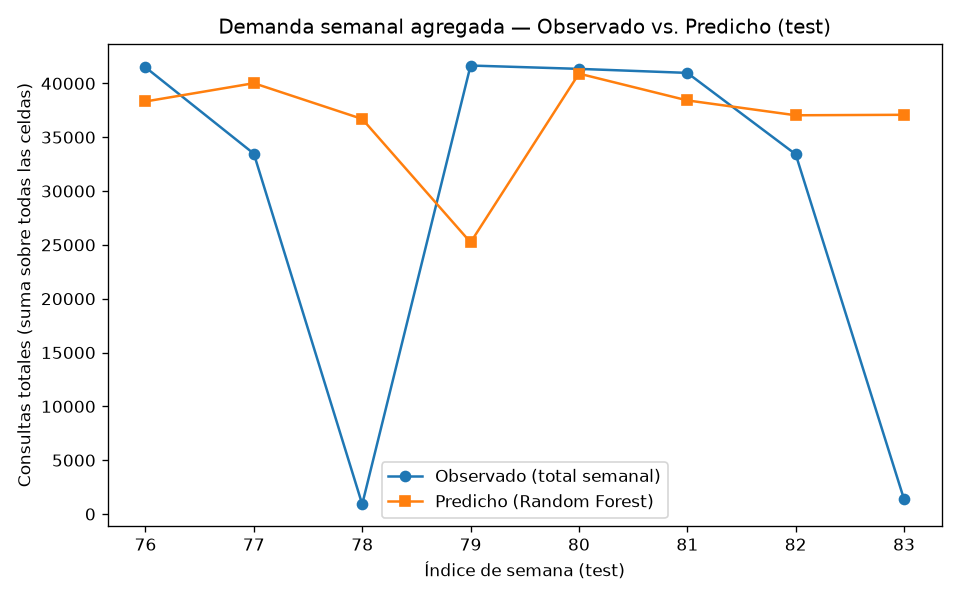
\includegraphics[width=0.7\textwidth]{imagenes/fig_weekly_demand_test.png}
  \fuente{Elaboración propia, a partir de \var{22_results_analysis.py}. Las semanas
  2024-W18 y 2024-W23 (parciales, sección~\ref{sec:semanas-parciales}) explican los mayores
  desvíos agregados de la serie.}
\end{figure}

\subsubsection{Importancia de variables}
\label{sec:importancia-variables}

Las variables autorregresivas dominan la importancia en Random Forest y XGBoost
(\var{roll_mean4_n_queries_orig} explica el 97,9~\% de la reducción de impureza en
Random Forest), coherente con la fuerte autocorrelación semanal de la demanda documentada en
la sección~\ref{sec:cobertura-temporal}.

\begin{figure}[htbp]
  \centering
  \caption{Importancia de variables (Gini), Random Forest}
  \label{fig:importancia-rf}
  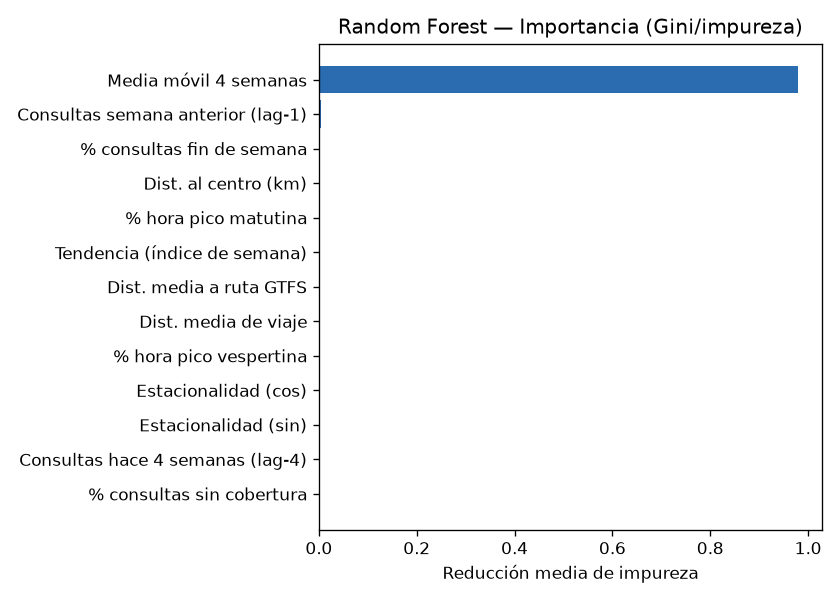
\includegraphics[width=0.65\textwidth]{imagenes/fig_feature_importance_rf.png}
  \fuente{Elaboración propia, a partir de \var{20_feature_importance.py} ---
  \var{reports/03_modeling/03_feature_importance.md}.}
\end{figure}

La señal territorial es más relevante de lo que sugiere la importancia por ganancia: en
XGBoost, \var{dist_center_km} ocupa la octava posición por ganancia pero asciende al
tercer lugar por magnitud media de SHAP, un método de interpretabilidad que atribuye a cada
variable su contribución marginal a cada predicción individual. Lasso --que lleva 9 de 13
coeficientes a cero, actuando como selector de variables-- conserva precisamente
\var{dist_center_km} (coeficiente estandarizado $-0{,}424$),
\var{roll_mean4_n_queries_orig} ($+0{,}396$), \var{lag1_n_queries_orig}
($+0{,}187$) y \var{pct_uncovered_orig} ($-0{,}077$) como la señal independiente más
robusta, con signos coherentes con H1: mayor distancia al centro y mayor proporción sin
cobertura se asocian con menor demanda.

\subsection{¿Sirve el modelo para priorizar? Un criterio preinscrito, refutado}
\label{sec:sirve-para-priorizar}

Si el modelo no gana por precisión de valor de forma contundente, el argumento operativo que
quedaba era que, aunque no acertara la magnitud exacta, ordenara bien las celdas para efectos
de priorización territorial. Esta sección lo somete a prueba con un criterio \textbf{declarado
antes de observar los resultados}: el modelo sirve para priorizar si ordena mejor que la
media móvil de 4 semanas, con diferencia media positiva, signo consistente entre semanas y
una prueba pareada que no lo contradiga. Declarar el criterio de antemano es lo que distingue
un hallazgo de una racionalización posterior, precisamente porque la comparación podía salir
en contra.

\textbf{El criterio no se cumple.} Promediando sobre las 6 semanas completas de prueba (se
excluyen las semanas parciales de la sección~\ref{sec:semanas-parciales}):

\begin{table}[htbp]
  \centering
  \caption{Métricas de ordenamiento territorial, promedio de las 6 semanas completas de prueba}
  \label{tab:ranking-metricas}
  \interlineadoSimple
  \begin{tabular}{lrrr}
    \toprule
    \textbf{Método} & \textbf{vRecall@20} & \textbf{NDCG@20} & \textbf{$\tau$-b de Kendall} \\
    \midrule
    \textbf{Base: media móvil 4 sem.} & \textbf{0,996} & \textbf{0,999} & \textbf{0,853} \\
    Random Forest & 0,995 & 0,996 & 0,850 \\
    XGBoost & 0,993 & 0,997 & 0,843 \\
    Base: persistencia ($t-1$) & 0,983 & 0,994 & 0,800 \\
    Ranking aleatorio (piso) & 0,022 & 0,104 & 0,001 \\
    \bottomrule
  \end{tabular}
  \fuente{Elaboración propia, a partir de \var{26_ranking_metrics.py} ---
  \var{reports/04_evaluation/04_ranking_metrics.md}.}
\end{table}

Random Forest no supera a la media móvil de 4 semanas en ninguna de las 6 semanas completas,
en ninguna de las métricas de ordenamiento evaluadas: el recuento de volumen alcanzable en
las 20 celdas elegidas (vRecall@20, la métrica principal, continua e insensible a empates), la
calidad del orden ponderada por posición (NDCG@20, calculada sobre relevancia logarítmica
porque con conteos crudos todos los métodos saturan por encima de 0,97) y la correlación de
rangos ($\tau$-b de Kendall, restringida a las celdas con demanda media de entrenamiento
$\geq 5$ para no dejar que domine el 76,6~\% de observaciones con demanda nula en prueba).
Ningún corte rescata la comparación: ni el estrato de demanda media (correlación de Spearman
0,957 contra 0,958 de la base) ni el ranking de los cambios semana a semana (0,458 contra
0,514, también a favor de la base).

\begin{figure}[htbp]
  \centering
  \caption{Comparación de métricas de ordenamiento por método y semana}
  \label{fig:ranking-comparacion}
  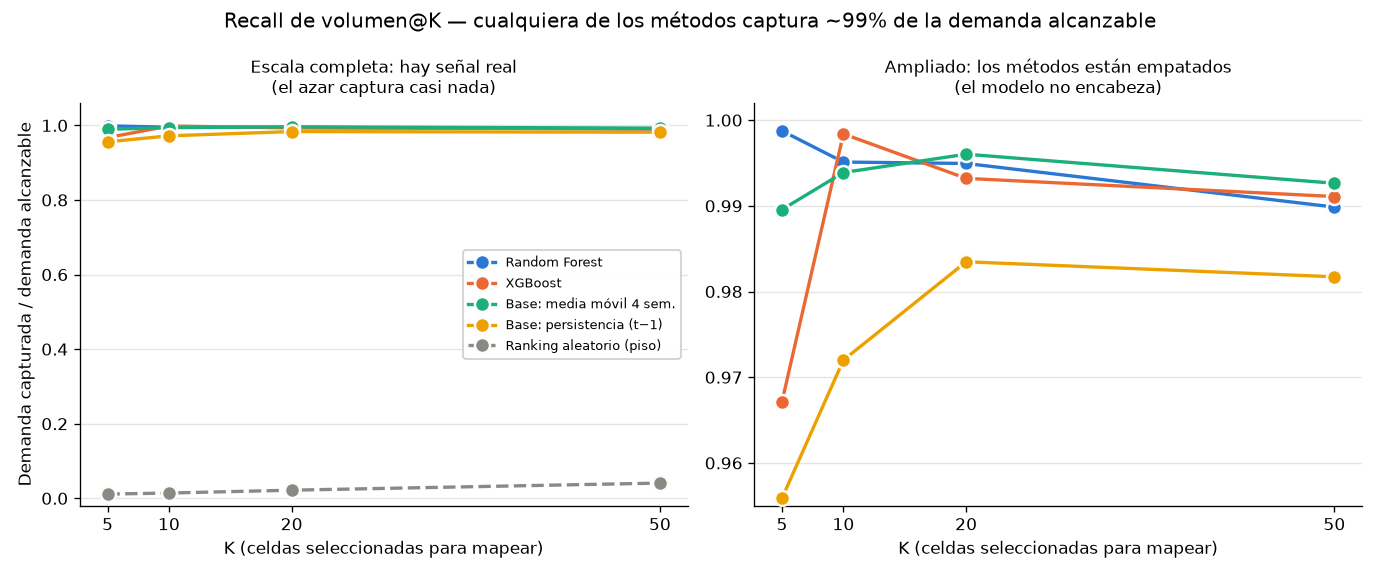
\includegraphics[width=0.75\textwidth]{imagenes/fig_ranking_comparison.png}
  \fuente{Elaboración propia, a partir de \var{26_ranking_metrics.py}.}
\end{figure}

\begin{figure}[htbp]
  \centering
  \caption{Cómo se calcula e interpreta la métrica de priorización}
  \label{fig:ranking-explicador}
  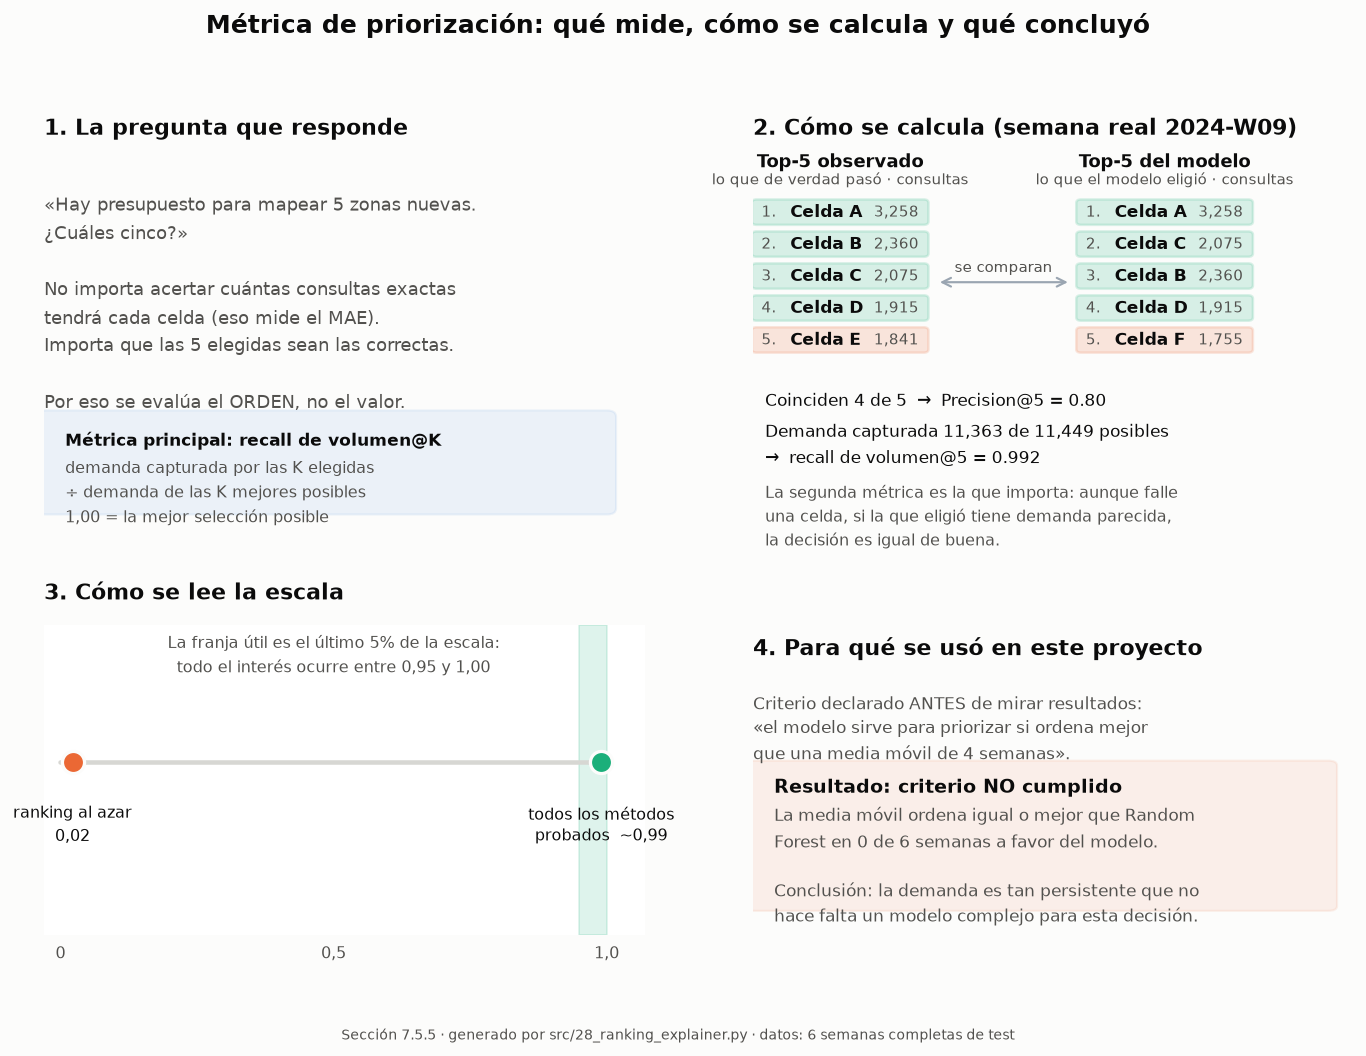
\includegraphics[width=0.75\textwidth]{imagenes/fig_ranking_explainer.png}
  \fuente{Elaboración propia, a partir de \var{28_ranking_explainer.py}.}
\end{figure}

Un coeficiente de correlación de rangos alto --como el $\rho=0{,}877$ entre demanda
observada y predicha reportado en la sección~\ref{sec:interpretacion-resultados}-- es fácil
de obtener cuando la distribución subyacente está tan concentrada como aquí (Gini$=0{,}934$,
sección~\ref{sec:sensibilidad-h3}): el ordenamiento de celdas es casi invariante entre
semanas, de modo que cualquier estimador --incluida una media móvil, e incluso la
persistencia-- reproduce ese orden. Esa cifra mide que el modelo no destruye una señal
trivialmente disponible; no mide que aporte capacidad de ordenamiento propia, que es
justamente lo que esta comparación contra competencia refuta.

\textbf{Este resultado no debilita el trabajo, lo fortalece.} Se obtuvo con un criterio
declarado de antemano y una comparación que podía salir en contra, exactamente lo que
distingue un hallazgo de una racionalización posterior. La formulación correcta es que, para
decidir qué celdas mapear a un horizonte de una semana, no se justifica un modelo complejo:
una media móvil de cuatro semanas ordena igual o mejor, y es además transparente, barata de
operar y auditable. La contribución de este trabajo está en el pipeline reproducible, la
caracterización territorial y el diagnóstico de cobertura (H1), no en la superioridad de un
estimador de valor. El alcance de esta refutación es específico: vale para horizonte de una
semana; a horizontes mayores la media móvil envejece y el modelo podría mostrar ventaja, pero
esa prueba no se realizó --requeriría reconstruir los rezagos y reentrenar-- y queda
declarada como pendiente, no como ventaja supuesta.

\subsection{Selección y justificación del modelo final}
\label{sec:seleccion-final}

\textbf{Random Forest se selecciona como modelo final}, con un criterio explícito aplicado
en el siguiente orden: menor MAE de prueba entre los cuatro modelos ajustados (10,19); menor
brecha entre entrenamiento y prueba que XGBoost ($+8{,}00$ frente a $+11{,}76$); y único
modelo que supera de forma consistente a ambas líneas base. XGBoost se descarta pese a un MAE
de validación cruzada competitivo (4,17 frente a 3,58 de Random Forest): en el conjunto de
prueba resulta peor (13,85) que la propia línea base estacional (11,05) --un caso concreto de
por qué no debe elegirse un modelo por su posición en una única métrica de validación. Haber
sido el primer modelo ejecutado no cuenta como criterio, exigencia explícita de la guía de la
materia.

La selección se sostiene también en interpretabilidad y costo computacional: Random Forest no
requiere las precauciones de extrapolación que exigirían Ridge o Lasso en producción, y su
tiempo de entrenamiento es compatible con la cadencia de reentrenamiento trimestral propuesta
en la sección~\ref{sec:despliegue}. Su ventaja frente a la línea base es real y
estadísticamente significativa donde más importa operativamente (H2), aunque --como se
estableció en la sección~\ref{sec:sirve-para-priorizar}-- esa ventaja no se traduce en una
mejor capacidad de ordenamiento territorial que una media móvil simple.
